\beginsong{Miruschka}[wuw={mündlich überliefert}, bo={236}, pfiii={20}]

\markboth{\songtitle}{\songtitle}

\beginverse
\endverse

\centering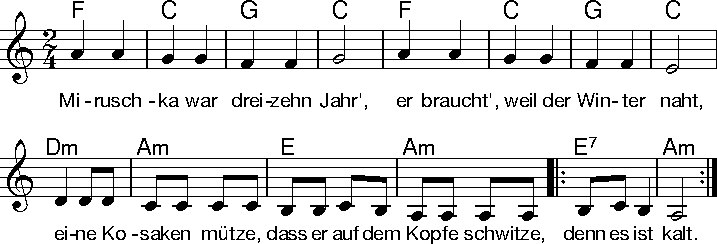
\includegraphics[width=1\textwidth]{Noten/Lied065.pdf}	

\beginverse
\[F]Seine \[C]gute \[G]Babusch\[C]ka \[F]schenkt ihm \[C]eine \[G]Tschapotsch\[C]ka.
\endverse

\beginchorus
\[Dm]Eine Ko\[Am]sakenmütze, \[E]dass er auf dem \[Am]Kopfe schwitze, \lrep \[E7]denn es ist \[Am]kalt. \rrep
\endchorus

\beginverse
^Eines ^Tages, ^welch ein ^Schreck, ^ach da ^war die ^Tschapka ^weg.
\endverse

\beginverse
^Väter^chen, wo ^ist mein ^Hut? ^Kalter ^Kopf, der ^tut nicht ^gut. 
\endverse

\beginverse
^Traurig ^sucht er ^sie im ^Wald ^und es ^ist schon ^bitter^kalt.
\endverse

\beginverse
^Immer ^kälter ^wird's im ^Tann ^und er ^macht ein ^Feuer ^an.
\endverse

\beginverse
^Vorne ^hat er ^große ^Hitze, ^wenn er ^doch auch ^hinten ^schwitze.
\endverse

\beginverse
^Und so ^macht sich ^Mirusch^mann ^hinter ^sich ein ^Feuer ^an.
\endverse

\beginverse
^Traurig ^starrt er ^in die ^Glut, ^da ge^friert vor ^Schreck sein ^Blut.
\endverse

\beginverse
^Mirusch^ka ist ^hell ent^setzt, ^hinter ^ihm steht ^Meister ^Petz.
\endverse

\beginverse
^Mirusch^ka flieht ^aus dem ^Banne ^und er^klettert ^eine ^Tanne.
\endverse

\beginverse
^Doch der ^Ast zer^bricht mit ^Knall, ^Mirusch^ka kommt ^schwer zu ^Fall.
\endverse

\beginverse
^Auf des ^Bären ^Nase ^drauf, ^der gibt ^seinen ^Geist gleich ^auf.
\endverse

\beginverse
^Mirusch^ka, der ^lachte ^hell: ''^Hei, ich ^hab' mein ^Mützchen^fell.''
\endverse

\endsong

\beginscripture{}
Babuschka = Weib; Tschapotschka = Kappe/Mütze
\endscripture

\begin{intersong}

\end{intersong}